\section{PPF Design and Architecture}
\label{Arch}
% Really need a high-level overview of the technique before you start
% talking about tables!

\begin{figure}
  \begin{center}
  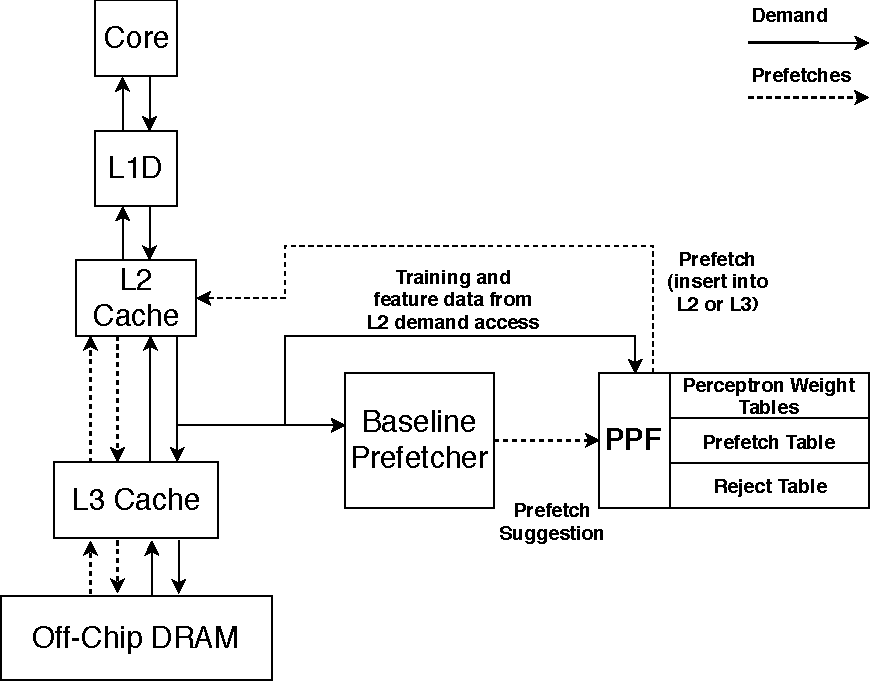
\includegraphics[width=8cm]{PPF_Hierarchy}
  \caption{PPF Architecture in the Memory Hierarchy}
  \label{fig:PPF_Hierarchy}
  \end{center}
\end{figure}

It can be beneficial to allow a prefetcher to speculate as deeply as
possible. Often, some useful prefetches are generated long after the
confidence of the prefetcher has fallen below a point, after which the
performance degrades, due to the increase of inaccurate prefetches. However,
in order to allow deep speculation in the prefetcher, inaccurate prefetches
must be filtered out. We propose to leverage perceptron-based learning as a
mechanism to differentiate between potentially useful deeply speculated
prefetches and likely not-useful ones. The Perceptron Prefetch Filter (PPF) is
placed between the prefetcher and the prefetch insertion queue, as illustrated
in figure~\ref{fig:PPF_Hierarchy}, to prevent not-useful prefetches from
polluting the higher levels of the memory hierarchy.

Perceptron learning is a light-weight mechanism to pull together disparate
forms of information and synthesize a decision from them. Our work considers
a number of features corresponding to a prefetch, such as speculation depth,
page address and offset, and uses this information as the inputs to our
perceptron-based filter, in order to predict the usefulness of a prefetch. In
the remainder of this section, we discuss our proposed technique: PPF. It
enhances a base prefetcher, by filtering out not-useful prefetches. PPF is a
generalized prefetch filtering mechanism that may be adapted to any prefetcher
with appropriate modifications.

\begin{figure}[ht]
  \begin{center}
  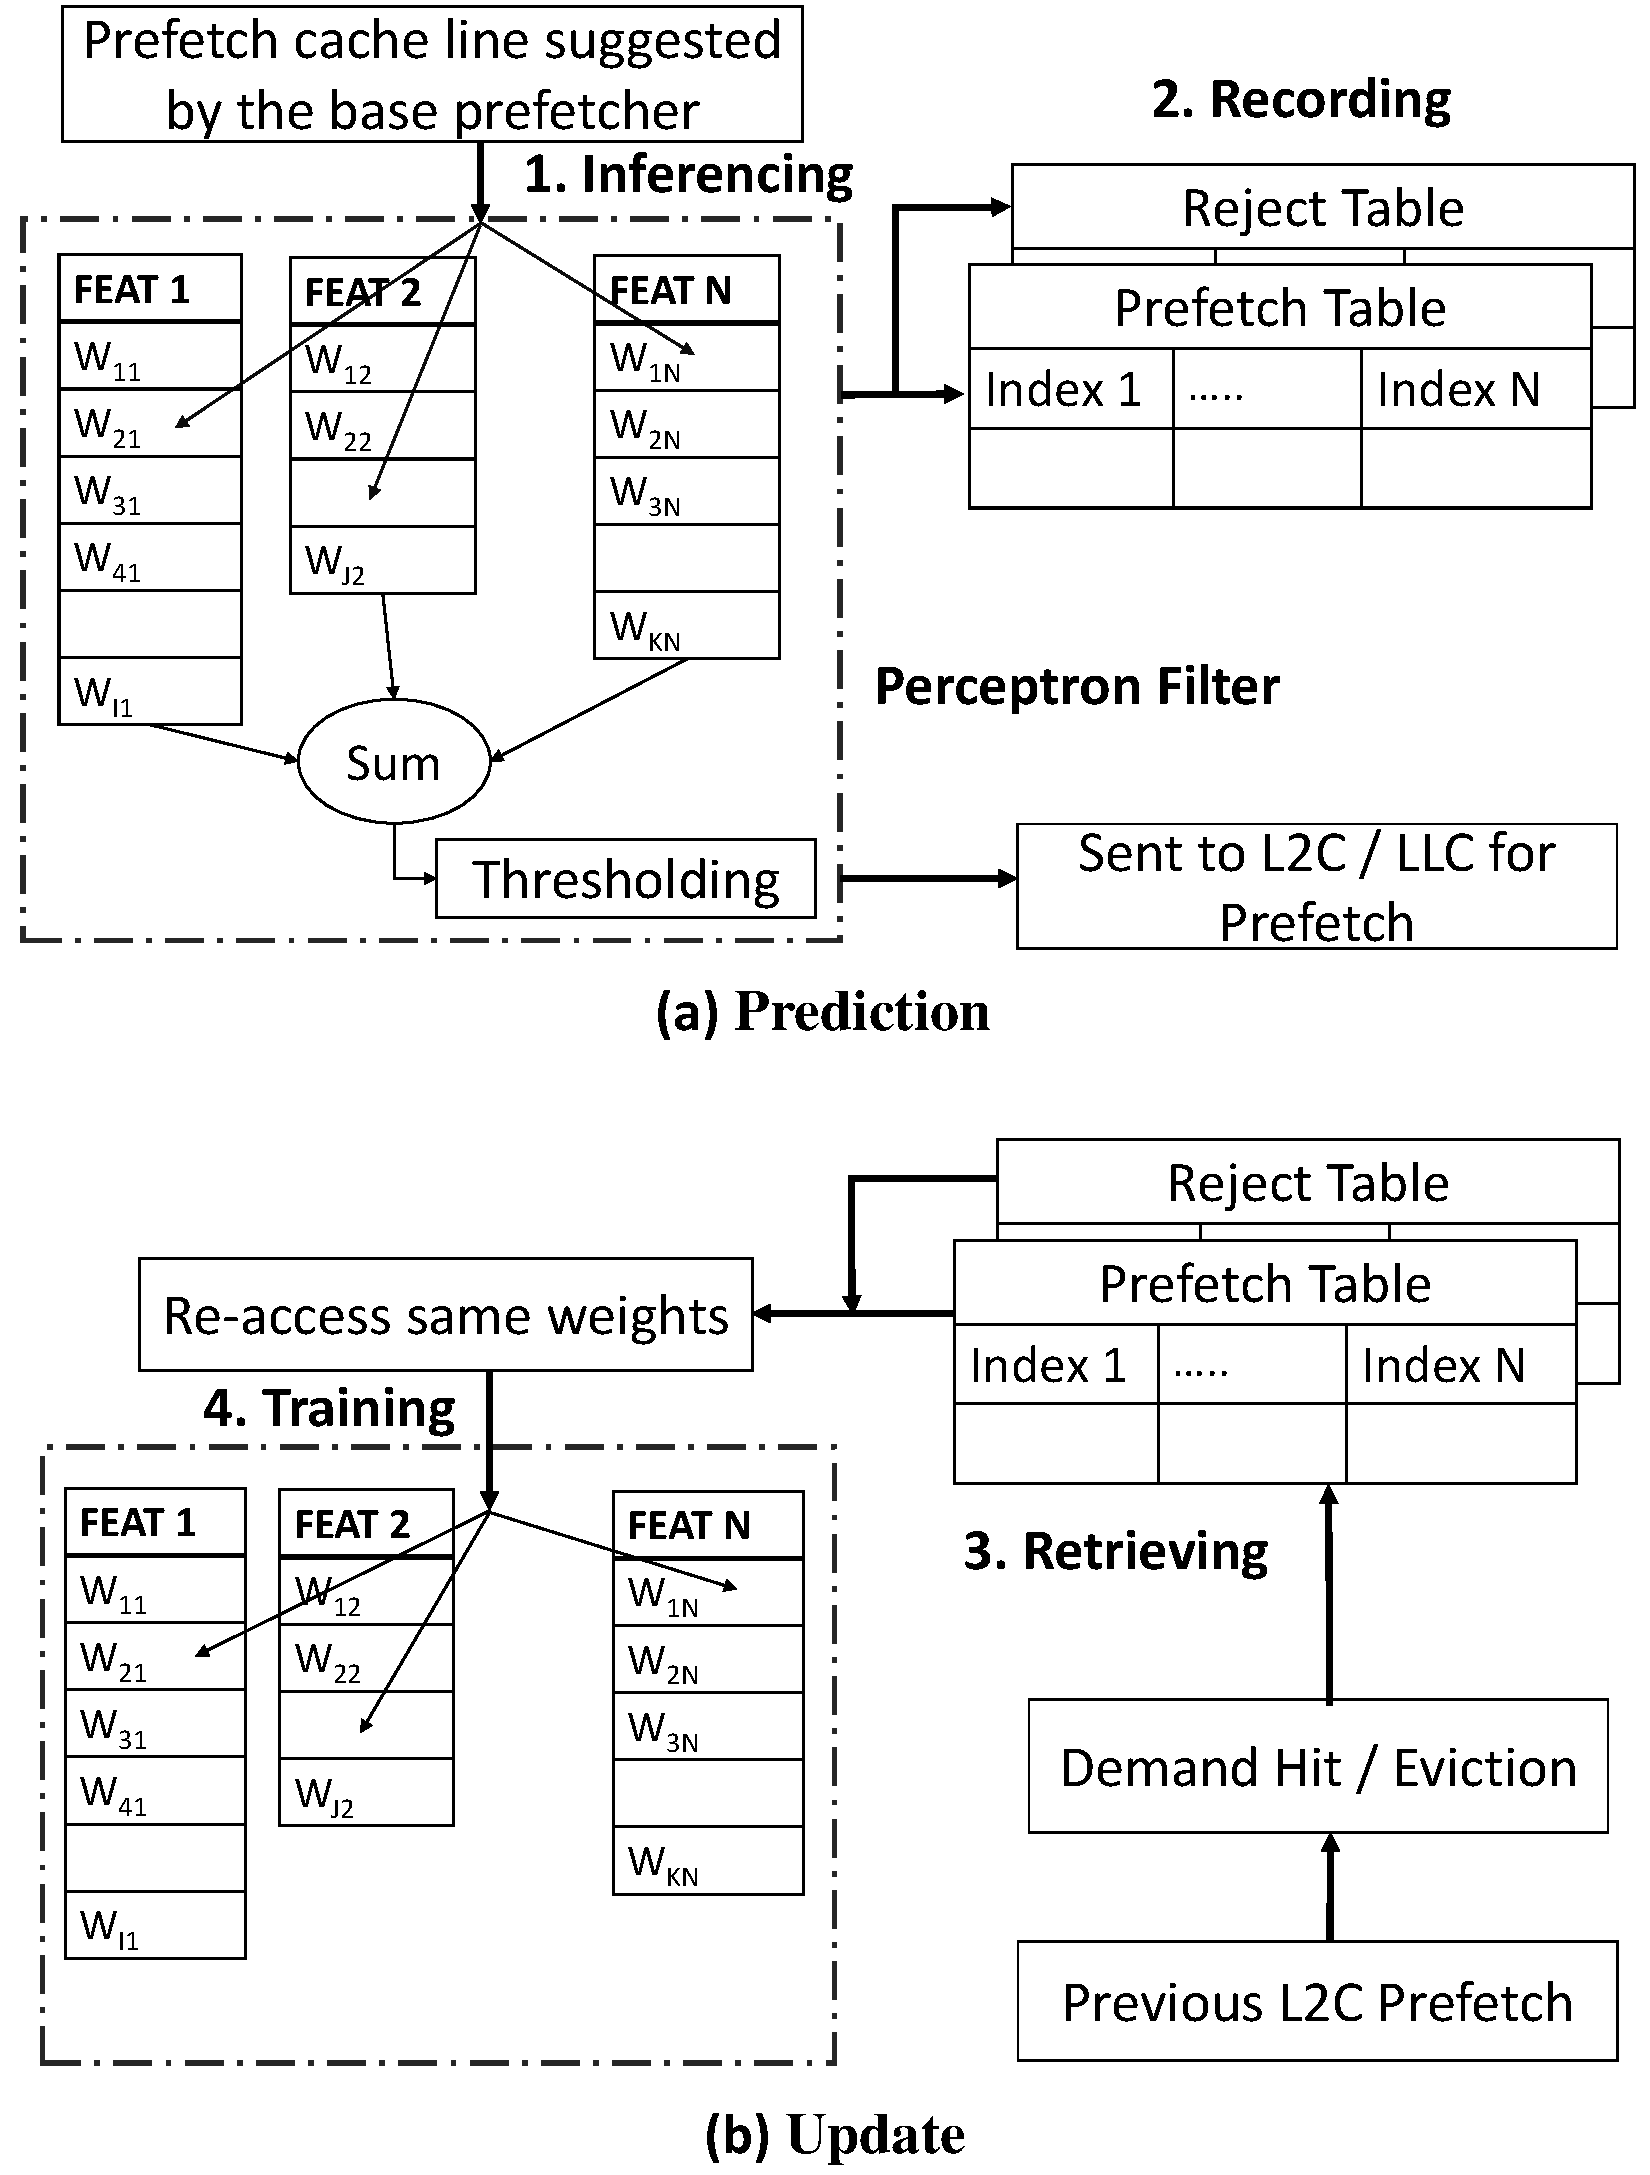
\includegraphics[width=\columnwidth]{Datapath_Separate}
  \caption{PPF Data Path and Operation}
  \label{fig:PPF_Datapath}
  \end{center}
\end{figure}

\subsection{The Perceptron Filter}
\label{Arch-Perceptron}
%\pg{rewrite this section as talking to the figures and walking through them}

Figure~\ref{fig:PPF_Datapath} shows the required structures of PPF, as well as
the steps followed to filter out not-useful prefetches. The filter is
organized as a set of tables, where each entry in the tables holds a
\textit{weight}. For a configuration of PPF using $N$ number of features, $N$
different tables of weights are needed. Each feature is used to index a
distinct table. The number of entries of each table varies according to their
corresponding feature, hence, different number of bits are needed to index
different tables. Each weight is a 5-bit saturating counter ranging from -16
to +15. We found that having 5-bit weights provide a good trade-off between
accuracy and area. A detailed explanation of the storage overhead of PPF can
be found in Section~\ref{Method-Overheads}.\\

\noindent{\textbf{Inferencing}\\
%ETG:is this like an explanation of how prefetching happens? 
%EB: I see this as a short context of the datapath leading to the perc filter.
The base prefetcher is triggered on every demand access to the L2 Cache. At
this point, it has the opportunity to trigger a prefetch. If it decides to do
so, it will also need to decide how many cache blocks to prefetch. These
blocks can be either placed in the L2 or L3 cache according to the confidence
of the prefetching mechanism. Once the base prefetcher is triggered, the
suggested prefetch candidates are fed to the perceptron filter to determine
the usefulness of these prefetches. The filter makes the decision to issue
the prefetch suggestions from the base prefetcher. To make the decision, each
feature corresponding to a suggested prefetch is used to index a table and all
the corresponding weights are summed. The sum denotes the confidence value
for the suggested prefetch, and is thresholded against two different
magnitudes: $\tau_{hi}$ and $\tau_{lo}$.

Prefetches whose sum exceeds $\tau_{hi}$ are placed into the L2 cache.
The higher confidence value hints the prefetch would be useful and should be
prioritized. A prefetch for which the features result in a confidence value
between $\tau_{lo}$ and $\tau_{hi}$ is allocated in the larger
LLC, as the filter is moderately confident of the future reuse of the cache
block, but not enough to possible pollute a significantly smaller L2.
Suggested prefetches for which the features lead to a confidence value lower
than $\tau_{lo}$ are not prefetched, as the low confidence value
represents that the perceptron has learn that similar set of features are
associated with non-useful prefetches. \newline

\noindent \textbf{Recording}\\
As shown in step 2 of figure~\ref{fig:PPF_Datapath} the prefetches that make
it through the inference stage are recorded in the ``Prefetch Table''. The
prefetch table is a 1,024-entry, direct mapped structure that contains all
metadata required to re-index the perceptron entries for training.

In addition to the prefetch table mentioned above, PPF also maintains a
1,024-entry direct-mapped ``Reject Table.'' If a prefetch suggestion is
rejected by the perceptron layer, it is logged into the reject table. The
table is used to train the perceptron to avoid false negatives \textit{i.e.},
cases where the prediction suggested to reject the prefetch but the prefetch
was proven to be useful based on the observed demand accesses to the L2. \\

\noindent{\textbf{Feedback and Data Retrieval}\\
When there is an eviction or a demand access to the L2, training for both the
base prefetcher and our filter mechanism is triggered. The address of the
cache block that triggered training is used to index both the Prefetch and
Reject tables. 10 bits of the address are used to index tables, and another 6
bits to perform tag matching. Once the base prefetcher has suggested a
prefetch request, the corresponding features are used to index the tables of
weights. \newline

% Which bits? are the tables accesses sequentially?

\noindent{\textbf{Training}\newline
The address from the demand request triggering the training is looked up in
both tables. If the address is in the prefetch table and marked as valid, this
hints the previous prediction was correct and this is a useful prefetch. We
compute the sum of the corresponding weights. If the sum falls below a
specific threshold, training occurs and the corresponding weights are adjusted
accordingly. These thresholds are introduced in order to avoid over-training,
helping the filter adapt quickly to changes in memory behavior. These
thresholds are referred to as $\theta_p$ and $\theta_n$, 
respectively for the positive and negative values of training saturation.

On a cache block eviction, we look up the corresponding address in the
prefetch table. If there is a valid entry with this address, the filter made a
misprediction. The block was allocated in the L2 with a prefetch request that
the filter should have categorized as a useless prefetch. Thus, the
corresponding features of the prefetch request that cause these block to be
placed in the cache are used to index the tables of weights, and those weights
are adjusted accordingly.

%wait at the same time or no?
%Yes, and they are mutex cases

Parallel to accessing the prefetch table, on a demand access, the reject table
is accessed. Before the demand access triggers the next set of prefetches, the
reject table is checked for a valid entry. A hit means that the corresponding
cache block was initially suggested by the base prefetcher, but wrongly
rejected by the perceptron filter. The perceptron filter learns from this and
makes use of the corresponding features associated to the original prefetch
request, which are stored in the reject table, to index the weights tables and
adjust the weights accordingly.

Prior work in this domain lacks the knowledge of which cache blocks should have 
been prefetched, but were not. The implementation of the reject table,
allows us to have this information, which can be use to further optimize
our prefetching mechanism.

%Gino: rephrase below?
%The Perceptron Filter is organized as tables of perceptron weights, with a
%separate table of weights for each feature. For a design using `N' number of
%features, its weights will be arranged in $N$ different tables. Each feature's
%value is used to index into the corresponding table. Since each table is
%indexed independently, different numbers of bits can be used for indexing,
%thus giving each table a different size. The variable indexing can be
%determined by studying the features and fine-tuning them empirically to
%achieve a good accuracy versus hardware overhead trade-off. Exact details of
%our PPF implementation are given under ``Area Overheads'' in
%Section~\ref{Method-Overheads}. %
%%\pg{this whole ``bits'' discussion belongs in implementation not here IMHO}
%%[EB] Resolved
%
%A single entry in the table corresponds to a perceptron weight. Each weight
%is a 5 bit counter saturating at -16 and +15 and initialized to zero at the
%beginning of a program's execution. We observed empirically that 5 bits of
%index achieves a good trade-off between hardware overheads and accuracy.
%
%%\pg{the fact that its nine is again implementation details}
%% [EB] Resolved
%
%% \pg{The word ChampSim should not appear in this part of the paper at
%%  all. Remember you are describing how to build this in the general
%%  case...} 
%% [EB] Resolved
%
%\begin{figure}
%  \begin{center}
%  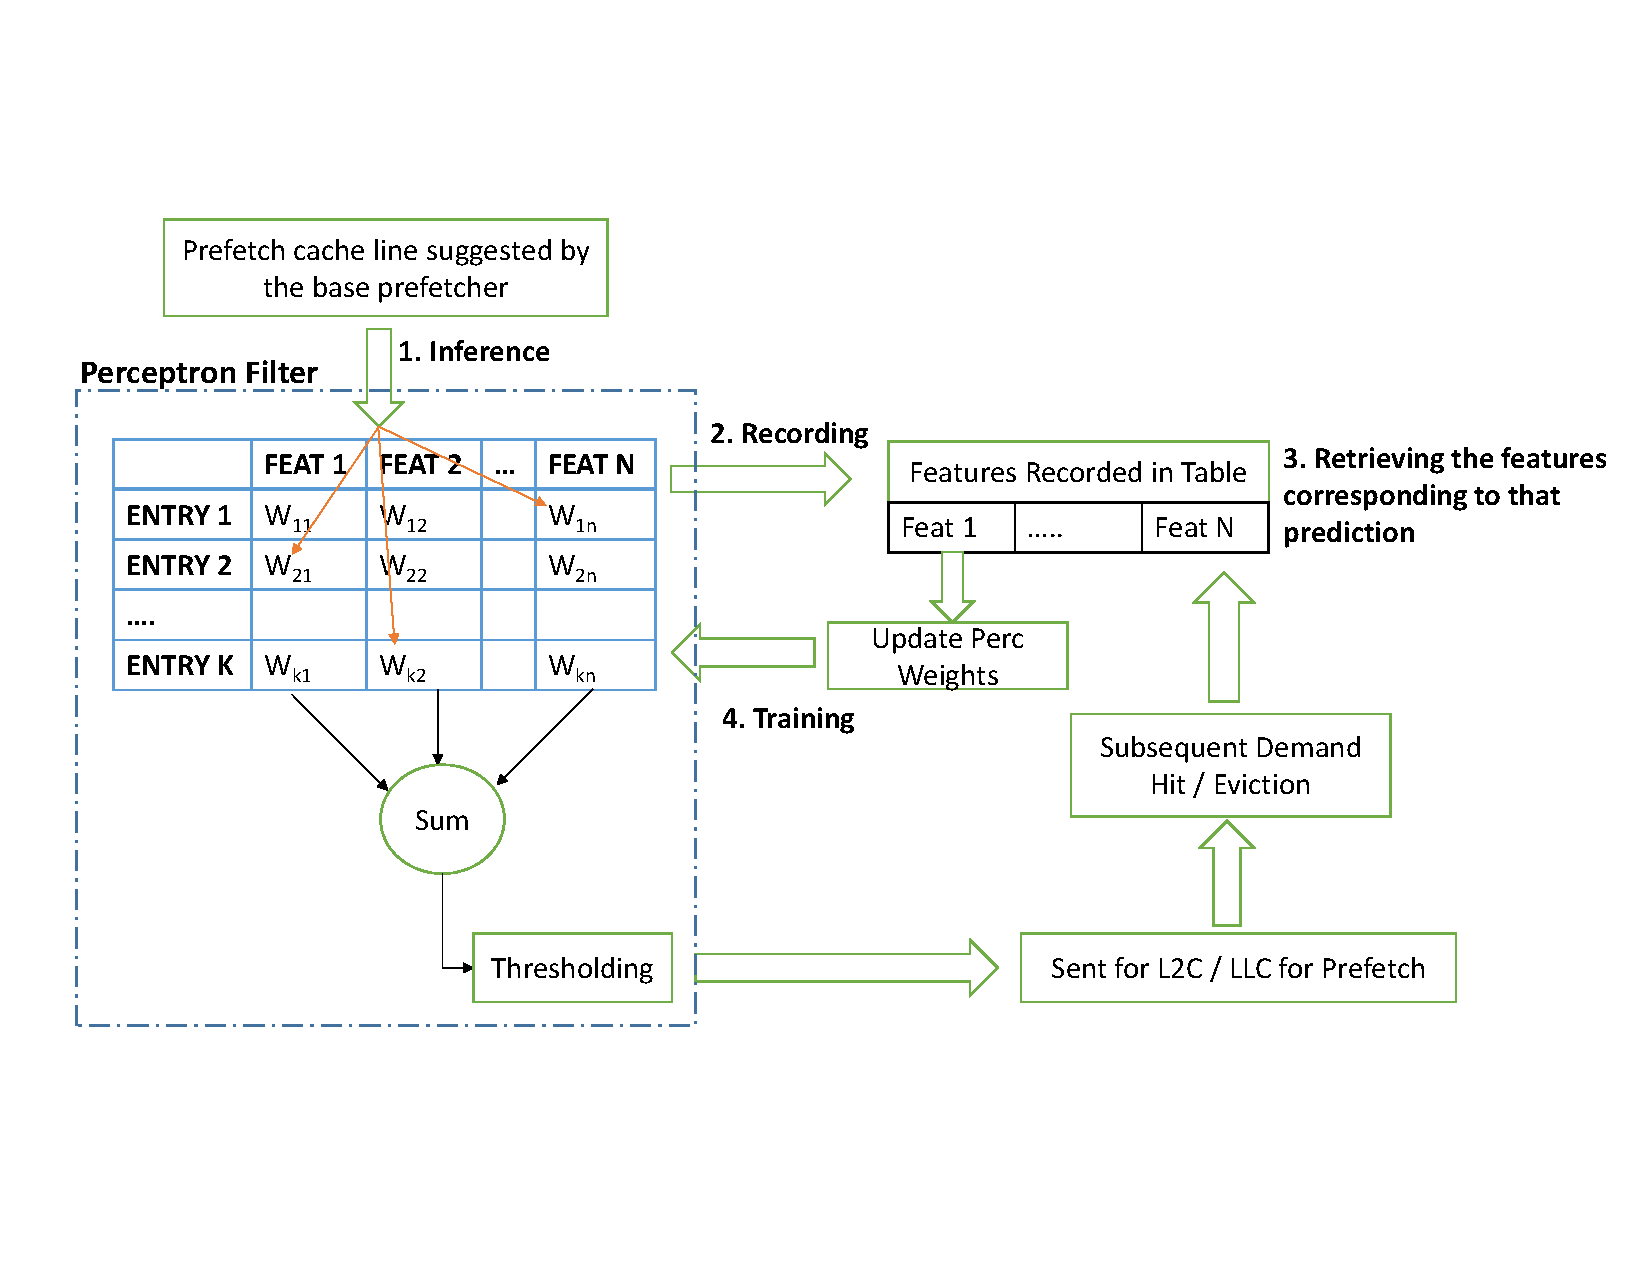
\includegraphics[width=9cm]{Datapath.pdf}
%    \label{fig:PPF_Datapath}
%  \caption{PPF Data Path and Operation}
%  \end{center}
%\end{figure}
%
%\textbf{Inference}\newline The prefetcher is triggered on every L2 cache
%demand access.  At that point, the base prefetcher has the option to perform a
%prefetch -- if it does, then it has a choice of how many cache lines to
%prefetch.  The suggested prefetches can be either placed in the L2 cache or
%the last-level cache based on the prefetcher's internal confidence mechanism.
%
%When the base prefetcher is triggered, it begins to suggest candidates for
%prefetching.  All suggested prefetches are passed through the perceptron
%filter to decide whether they are qualified for final prefetching.  The filter
%decides whether to prefetch a candidate by looking at the microarchitectural
%state, \textit{i.e.} the features, at that instant.  Each feature is hashed to
%form an index into a table of up to 4,096 entries dedicated to that feature.
%
%Once all the weights are retrieved, they are summed and compared to a preset
%threshold, PERC\_ THRESHOLD\_LO.  Only prefetch candidates with perceptron sum
%higher than the threshold qualify for prefetching.  The prefetches that
%qualify through the perceptron stage are recorded in the ``Prefetch Table''.
%The prefetch table is a 1,024-entry, direct mapped structure that contains all
%metadata required to re-index the perceptron entries for training.  When the
%feedback of the current prefetched line is available at a later stage, the
%stored data is used to train the perceptron.
%
%%\pg{this discussion below has redundancy and doesn't flow well.
%%  Rework it}
%
%Each feature's confidence contributes to the final decision of whether to
%prefetch a cache line, with the summation of all features' confidences
%denoting the overall confidence for a prefetch.  The final sum is compared
%against two thresholds: PERC\_THRESHOLD\_HI and  PERC\_ THRESHOLD\_ LO to
%decide the placement of the data in the cache hierarchy. Prefetches that have
%a confidence above the higher threshold are placed into the L2 cache since the
%observed features strongly recommend  the prefetch. A prefetch that results in
%a confidence between PERC\_ THRESHOLD\_ LO and PERC\_ THRESHOLD\_ HI are
%placed in the larger last level cache, as the filter is moderately confident
%of the cache line's use, but seeks to reduce pollution in the smaller L2
%cache. Finally, the remaining prefetches that are below the lower threshold
%are not prefetched due to a lack of correlation between the current observed
%features and the prediction from the base prefetch engine.
%
%In addition to the prefetch table mentioned above, PPF also maintains a
%``Reject Table.''  The reject table is a 1,024-entry direct-mapped table.
%If a prefetch suggestion is rejected by the perceptron layer, it is logged
%into the reject table.  The table is used to train the perceptron to avoid
%false negatives \textit{i.e.}, cases where prediction was to reject the
%prefetch but the prefetch would have been useful.
%
%%As previously stated all the metadata describing the program state at the
%%instant of prefetching is stored in the Prefetch Table or the Reject Table.
%%This information is useful when the perceptron needs to be updated
%%subsequently.
%
%\textbf{Training}\newline In the prefetching environment, feedback for a
%prefetch is received whenever there is an eviction or a demand access from the
%L2 cache.  This action triggers training of the base prefetcher as well as the
%perceptron layer.  Training the perceptrons involves accessing the metadata
%that was stored in Prefetch Table or the Reject Table.  The cache lines
%address of the block being trained is used to access a table, using 10 bits of
%the address for indexing and another 6 bits to perform tag matching.  Once the
%values of the features at the time of prefetching is available, it is used to
%index into the perceptron weights table.
%
%If the demanded block that triggers the training was tagged as a valid
%prefetch in the prefetch table, then the earlier prefetch prediction was
%correct.  In that case the perceptron weights are incremented by 1 if the
%predicted sum does not cross a pre-defined threshold. These training
%thresholds are introduced to avoid overfitting of the perceptron weights to
%the given program behavior. These thresholds are referred to as
%POS\_UPDATE\_THRESHOLD ($\theta_p$) and NEG\_UPDATE\_THRESHOLD ($\theta_n$),
%respectively for the positive and negative values of training saturation.
%
%If a cache block eviction led to training and the corresponding valid entry is
%found in the prefetch table without the block being accessed, then the
%prediction made by the perceptron was wrong.  The perceptron should have
%ideally rejected the prefetch suggestion as a low-confidence prefetch.  Here
%the weights are decremented by 1 to reflect the misprediction. In either case,
%weights are saturated at -16 or +15.
%
%A secondary training mechanism also kicks in during demand fetches.  Before
%the demand access triggers the next set of prefetches, the reject table is
%checked for a valid entry.  A hit means that the corresponding cache line was
%initially suggested by the underlying prefetch engine, but rejected by the
%perceptron filter.  Thus, the perceptron should have been more confident about
%that particular prefetch.  Once such a scenario is identified, the values of
%the features at the time of prefetch is retrieved from the reject table.  The
%retrieved data is used to index into the various weights tables of the
%perceptron and the corresponding values are updated by +1, saturating between
%and -16 and +15.  This update reflects increased confidence for the prediction
%corresponding to that prefetch.
%
%This mechanism allows us to exploit a previously lost opportunity.  In prior
%perceptron based implementations, and in general, prefetching algorithms,
%there is usually no way of knowing the result of not prefetching a particular
%line.  Our two-step PPF architecture allows us to overcome that issue.

\subsection{Optimizing PPF for a Given Prefetcher}
\label{Arch-Generalizing}
The above discussion of PPF shows that it is highly modular and can be adapted
to be used over any base prefetcher for increased prefetch accuracy. Only 
two hooks are required between PPF and the baseline prefetcher.
The first is to make sure that all the prefetch candidates of the prefetcher
pass through the perceptron filter and if qualified, the metadata for
perceptron indexing be stored. The second is needed when the feedback of a
prior prefetch is available in form of a subsequent demand hit or cache
eviction. In that case, the stored metadata needs to be retrieved to update
the state of the perceptrons.

In general, PPF can be adapted to a new base prefetcher with only a
few modifications:\\
%
\textbf{Enhancing the Base Prefetcher:} By tuning down any internal thresholds
to increase its inherent aggressiveness. \\
%
\textbf{Inferencing and Storing:} All prefetch recommendations are tested
using the perceptron inferencing algorithm. The perceptron's output,
\textit{true} or \textit{false}, should be saved appropriately, along with all
metadata required for perceptron indexing. \\
%
\textbf{Retrieving and Training:} When feedback for a prefetch is available,
the previously stored metadata can be used to re-index into the perceptron
entries and increment or decrement the weights. \\
%
\textbf{Feature Selection:} Perceptrons essentially normalize contributions
from different features to get a single sum representing the final confidence.
So the perceptron learning can be as good as the set of features chosen.
Interestingly, this is what makes perceptron learning scalable, as it can
easily learn to incorporate newer information in the form of new features.
Some of the features we developed use information derived directly from
program execution, agnostic to the baseline prefetcher. Beyond that, the
feature set can be expanded to convey any useful information from the
prefetcher to the perceptron filter.

% %[EB] This statement fits better in the next section 'Features used by
% Perceptron' %The methodology explained in %Section~\ref{Method-Features}
% talks about developing a minimal feature %set for PPF.

%\pg{This should be more about how one should
%choose features than about what you did in the SPP implementation
%in particular. Rewrite as a guide on picking features.}
% [EB]: Hopefully this is general enough and not too redundant
